\section{Identifying close pairs of particles}
In the \PThreeM{} method, in addition to the mesh used in the PM algorithm (the \textit{potential mesh}), a second mesh (the \textit{chaining mesh}) is used.
The chaining mesh is sparser than the potential mesh.
Its sole purpose is to partition the space into cells so that particles ``close'' to the ones in a given cell can be found efficiently.
In this context, two particles are considered to lie close to one another if their separation is less than the cutoff radius.

The number of chaining mesh cells in a single dimension is given by $M_i = \lfloor L_i / r_e \rfloor$, where $L_i$ is the side length of the computational box ($i=1,2,3$).
This implies that the side length of a chaining mesh cell is $\text{HC}_i = L_i / M_i \geq r_e$.
Thus, for every particle $i$ in a given chaining cell $\mathbf{p}$, it is sufficient to search through the immediate neighborhood of $\mathbf{p}$ (cells adjacent to $\mathbf{p}$) to find all the particles within the cutoff radius from $i$.

In our program, the chaining mesh is implemented as a \textit{head-of-chain} (HOC) array, depicted in \autoref{fig:hoc}.
\begin{figure}[htp]
    \centering
    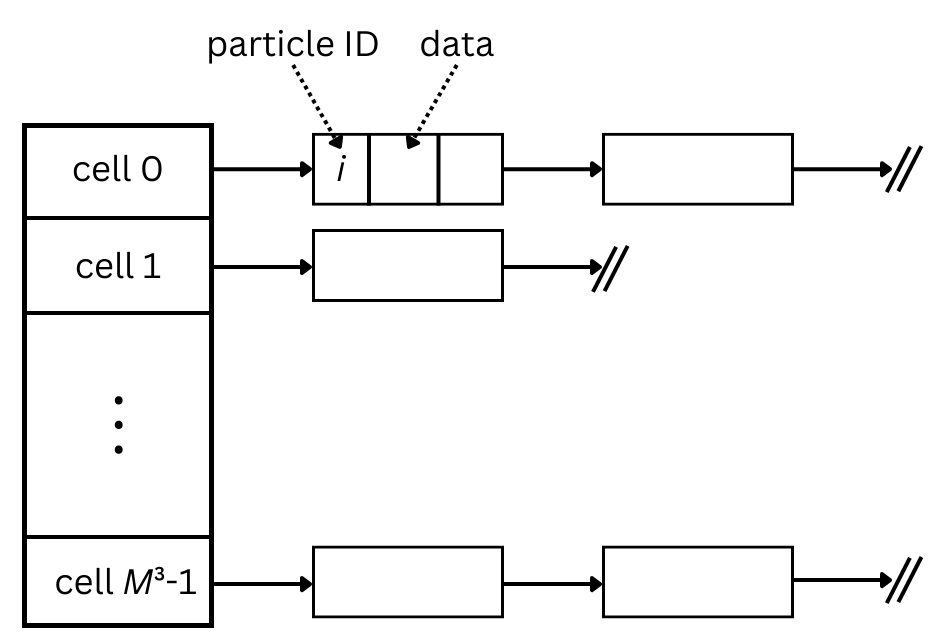
\includegraphics[scale=0.25]{chapters/p3m-method/img/hoc.png}
    \caption{Head-of-chain data structure used for mapping particles to their parent cells in the chaining mesh.
        Here $M_1=M_2=M_3 = M$.}
    \label{fig:hoc}
\end{figure}
The basic version of the HOC array is very cheap to build.
Given a particle at a point $\mathbf{x} = (x, y, z)$, we can determine in which chaining mesh cell $\mathbf{c}$ it lies by simply performing integer division on each of its coordinates, i.e., $\mathbf{c} = (\lfloor x / \text{HC}_1 \rfloor, \lfloor y / \text{HC}_2 \rfloor, \lfloor z / \text{HC}_3 \rfloor)$.
Then, to get a HOC table index $i$ corresponding to $\mathbf{c}$, standard index flattening is used.
Subsequently, a new linked-list node is allocated and inserted at the beginning of the list HOC[$i$].
The whole process is linear in the number of particles, and the array can be constructed anew at each time step without degrading performance.
In our implementation, additional savings are made by preallocating a memory pool large enough to store $N$ nodes of the linked lists and reusing it for the HOC array initialization.

A potential optimization discussed in \cite{Hockney1988} involves sorting each linked list by a selected particle coordinate, such as the $y$-coordinate.
This ordering enables early termination of the direct summation loop when the condition $y_j - y_i > r_e$ is met, effectively reducing unnecessary pairwise computations as particle $i$ ``is looking for its neighbors'' in a cell containing particles $j$.
Our experiments indicate that constructing the linked lists in sorted order is substantially more expensive than the unsorted variant.
This is to be expected; in the worst-case scenario where all particles are in a single chaining-mesh cell and are inserted into the list in decreasing order of $y$ coordinates, the complexity is $O(N^2)$.
For a system of 50{,}000 particles, incorporating $y$-sorting increased the HOC (head-of-chain) construction time from approximately 180 milliseconds to over 13{,}000 milliseconds, a 70-fold slowdown.
Despite this added cost, we observed no significant performance improvement in the short-range correction phase of the computation.
